% !TEX root = ../thesis.tex
% !TEX spellcheck = en-US

\clearpage
\section{Experiments}

\todo{Comparison one-vs-rest and one-vs-one against linear machine}
\todo{Visualizations and embeddings of data in 2D (and decision boundaries?)}
\todo{show T-SNE embeddings of doc2vec vectors}

\subsection{Effectiveness and Expressiveness of Statistical (Vector Space) Language Models}

\todo{say why using the sentence dataset here}
\todo{reference jupyter notebook here}
% http://localhost:8888/notebooks/thesis/experiments/vector-space-models/Vector%20Space%20Models.ipynb#Setup

As section~\ref{sec:vector-space-models} explains, a popular way to approach text classification and other tasks in natural language processing is to build a language model by creating explicit representations of the objects or entities to be processed in a vector space. Such vectors can be used as features for a learning algorithm. Depending on the representation they can also further meaning, such as to encode notions of similarity of associativity between the objects.

In order to determine effective vector space representations for the task of sentence classification, a set of experiments was carried out to study and compare different approaches. Each method was studied with regards to the effect of its hyper-parameters on effectiveness when producing an input space to different classifiers, but also time and memory requirements at training and inference time are taken into account \todo{actually discuss time and memory requirements}.

In order to compare the effectiveness for the sentence classification task as discussed in ?\todo{reference section here} each labelled document was transformed into a vector space representation using the different methods and then used for classification with a simple logistic regression classifier(\todo{link to logistic regression classifier explanation here}). Performance was then compared with regards to Matthews Correlation Coefficient for multi-class problems \todo{link MCC multi here} and Accuracy.

\subsubsection{Baselines Classifiers: Uniform and Stratified Guessing}
\label{subs:baselines-classifiers}

As a baseline for comparing the performance of classification two different guessing strategies were used, namely uniform and stratified guessing.
Uniform guessing refers to a predictor that samples from the given classes assuming a uniform distribution whereas stratified guessing takes the label distribution in the data as the underlying probability distribution.
Then both methods just sample from these distributions to produce ``predictions'', while ignoring the actual input data. Both, uniform and stratified guessing achieve a Matthews Correlation Coefficient score of around 0 (averaged over 1000 runs) as expected for such guessing strategies (see section~\ref{subs:informedness-markedness-mcc}). On the other hand the accuracy for uniform guessing is around 0.16 which corresponds to $1/\text{K}$ for the K classes and around 0.26 for stratified guessing which reflects the skew of the label distribution.
Figure~\ref{fig:exp-vector-space-conf-matrix-guessing} shows the confusion matrices for these baseline variants in absolute and normalized form which, revealing the properties of these guessing strategies.

\begin{figure}[h]
 % From http://localhost:8888/notebooks/thesis/experiments/vector-space-models/Vector%20Space%20Models.ipynb#Baseline:-Guessing-Strategies
    \centering
    \begin{subfigure}[b]{0.47\textwidth}
        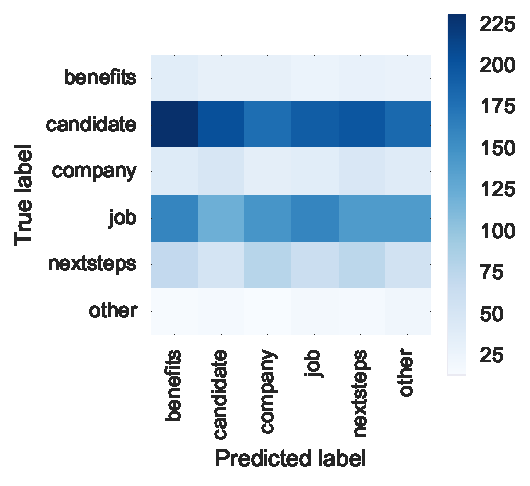
\includegraphics[width=\textwidth]{img/exp-vector-space-conf-matrix-guessing-uniform.pdf}
        \caption{Uniform, absolute}
      \label{fig:exp-vector-space-conf-matrix-guessing-uniform}
    \end{subfigure}
    ~
    %add desired spacing between images, e. g. ~, \quad, \qquad, \hfill etc.
    %(or a blank line to force the subfigure onto a new line)
    \begin{subfigure}[b]{0.48\textwidth}
        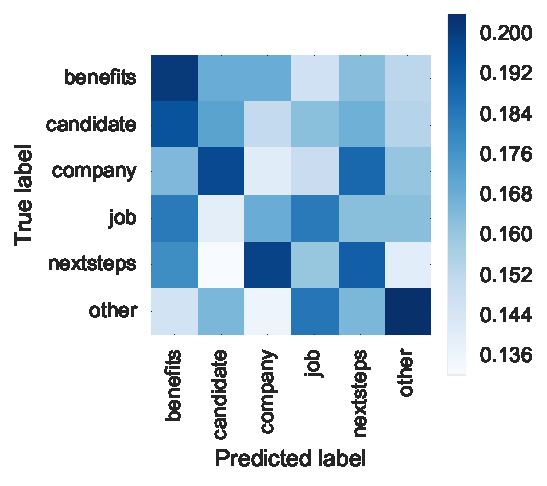
\includegraphics[width=\textwidth]{img/exp-vector-space-conf-matrix-guessing-uniform-normalized.pdf}
        \caption{Uniform, normalized}
        \label{fig:exp-vector-space-conf-matrix-guessing-uniform-normalized}
    \end{subfigure}
    ~
    \begin{subfigure}[b]{0.47\textwidth}
        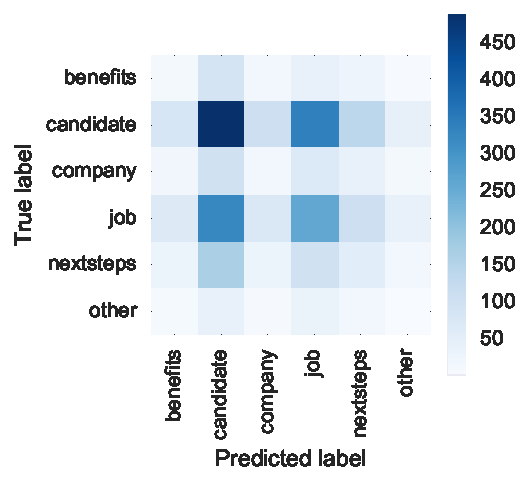
\includegraphics[width=\textwidth]{img/exp-vector-space-conf-matrix-guessing-stratified.pdf}
        \caption{Stratified, absolute}
        \label{fig:exp-vector-space-conf-matrix-guessing-stratified}
    \end{subfigure}
    ~
    %add desired spacing between images, e. g. ~, \quad, \qquad, \hfill etc.
    %(or a blank line to force the subfigure onto a new line)
    \begin{subfigure}[b]{0.48\textwidth}
        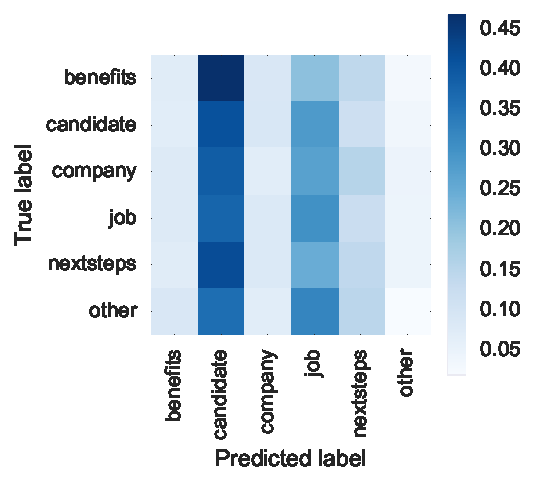
\includegraphics[width=\textwidth]{img/exp-vector-space-conf-matrix-guessing-stratified-normalized.pdf}
        \caption{Stratified, normalized}
        \label{fig:exp-vector-space-conf-matrix-guessing-stratified-normalized}
    \end{subfigure}
    \caption{Confusion matrices of uniform and stratified guessing strategies. }
  \label{fig:exp-vector-space-conf-matrix-guessing}
\end{figure}

\subsubsection{N-gram Language Models}

The first class of language models that was investigated for the task of multi-class classification are N-gram models that were explained in section~\ref{subs:n-gram-language-models}. As mentioned earlier this type of model relies on simple statistics makes for straightforward computation but at the same time comes at cost of expressiveness in terms of temporal dependencies between words.

As this approach has been studied for decades \todo{citation for first or review paper here?} there is quite an extensive amount of variants and thus hyper-parameters to tune. To compare the effects of these hyper-parameters for the different N-gram models a grid search was performed, searching over a large parameter space.

\begin{center}
  \begin{table}[h]
  \begin{tabular}{ l l l}
    \hline
    Parameter & Search Space N-grams Words & Search Space N-grams Characters \\
    \hline
    N-gram range & [1,1], [1,2], [1,3], [2,3], [3,3] & [1,5], [1,10], [5,10], [5,15] \\
    Stop words & English, None & N/A \\
    Vector size & 10, 100, 300 & 10, 100, 300 \\
    IDF & Yes, No & Yes, No \\
    Norm & L1, L2, None & L1, L2, None \\
    Sublinear TF & Yes, No & Yes, No \\
    \hline
  \end{tabular}
  \caption{Parameter search space for word and character level N-gram models}
\label{table:name}
  \end{table}
\end{center}



\todo{show influence of each parameter on the performance by fixing it to each value it can take and measuring the variance of the results? or by just showing the mean when fixing to one value}




\subsubsection{Distributed Language Models}

- word2vec averaged
- par2vec
- inversed baysian

%
% \subsection{Classification of paragraph labels}
%
% \subsection{Unsupervised label detection}
%
%
%
% \subsection{Classification of sentence labels}
%
% \subsubsection{Experiment 1: Feature Extraction through Vector Space Models}
%
% \subsubsection{N-gram models}
% \label{ngram-models}
%
%
%
% \subsubsection{Distributed Representations language models}
% \label{doc2vec}
%
% Following an approach proposed by \cite{Le:2014aa}, the rationale of this experiment was to find out it was possible to obtain a more expressive language model than the N-gram based methods described in \ref{ngram-models}.
%
% The idea is based
%
% \subsection{Neural Networks}
